%!TeX root=../pridetop.tex
\chapter[Chapter \thechapter]{}
	
\begin{figure}[t!]
\centering
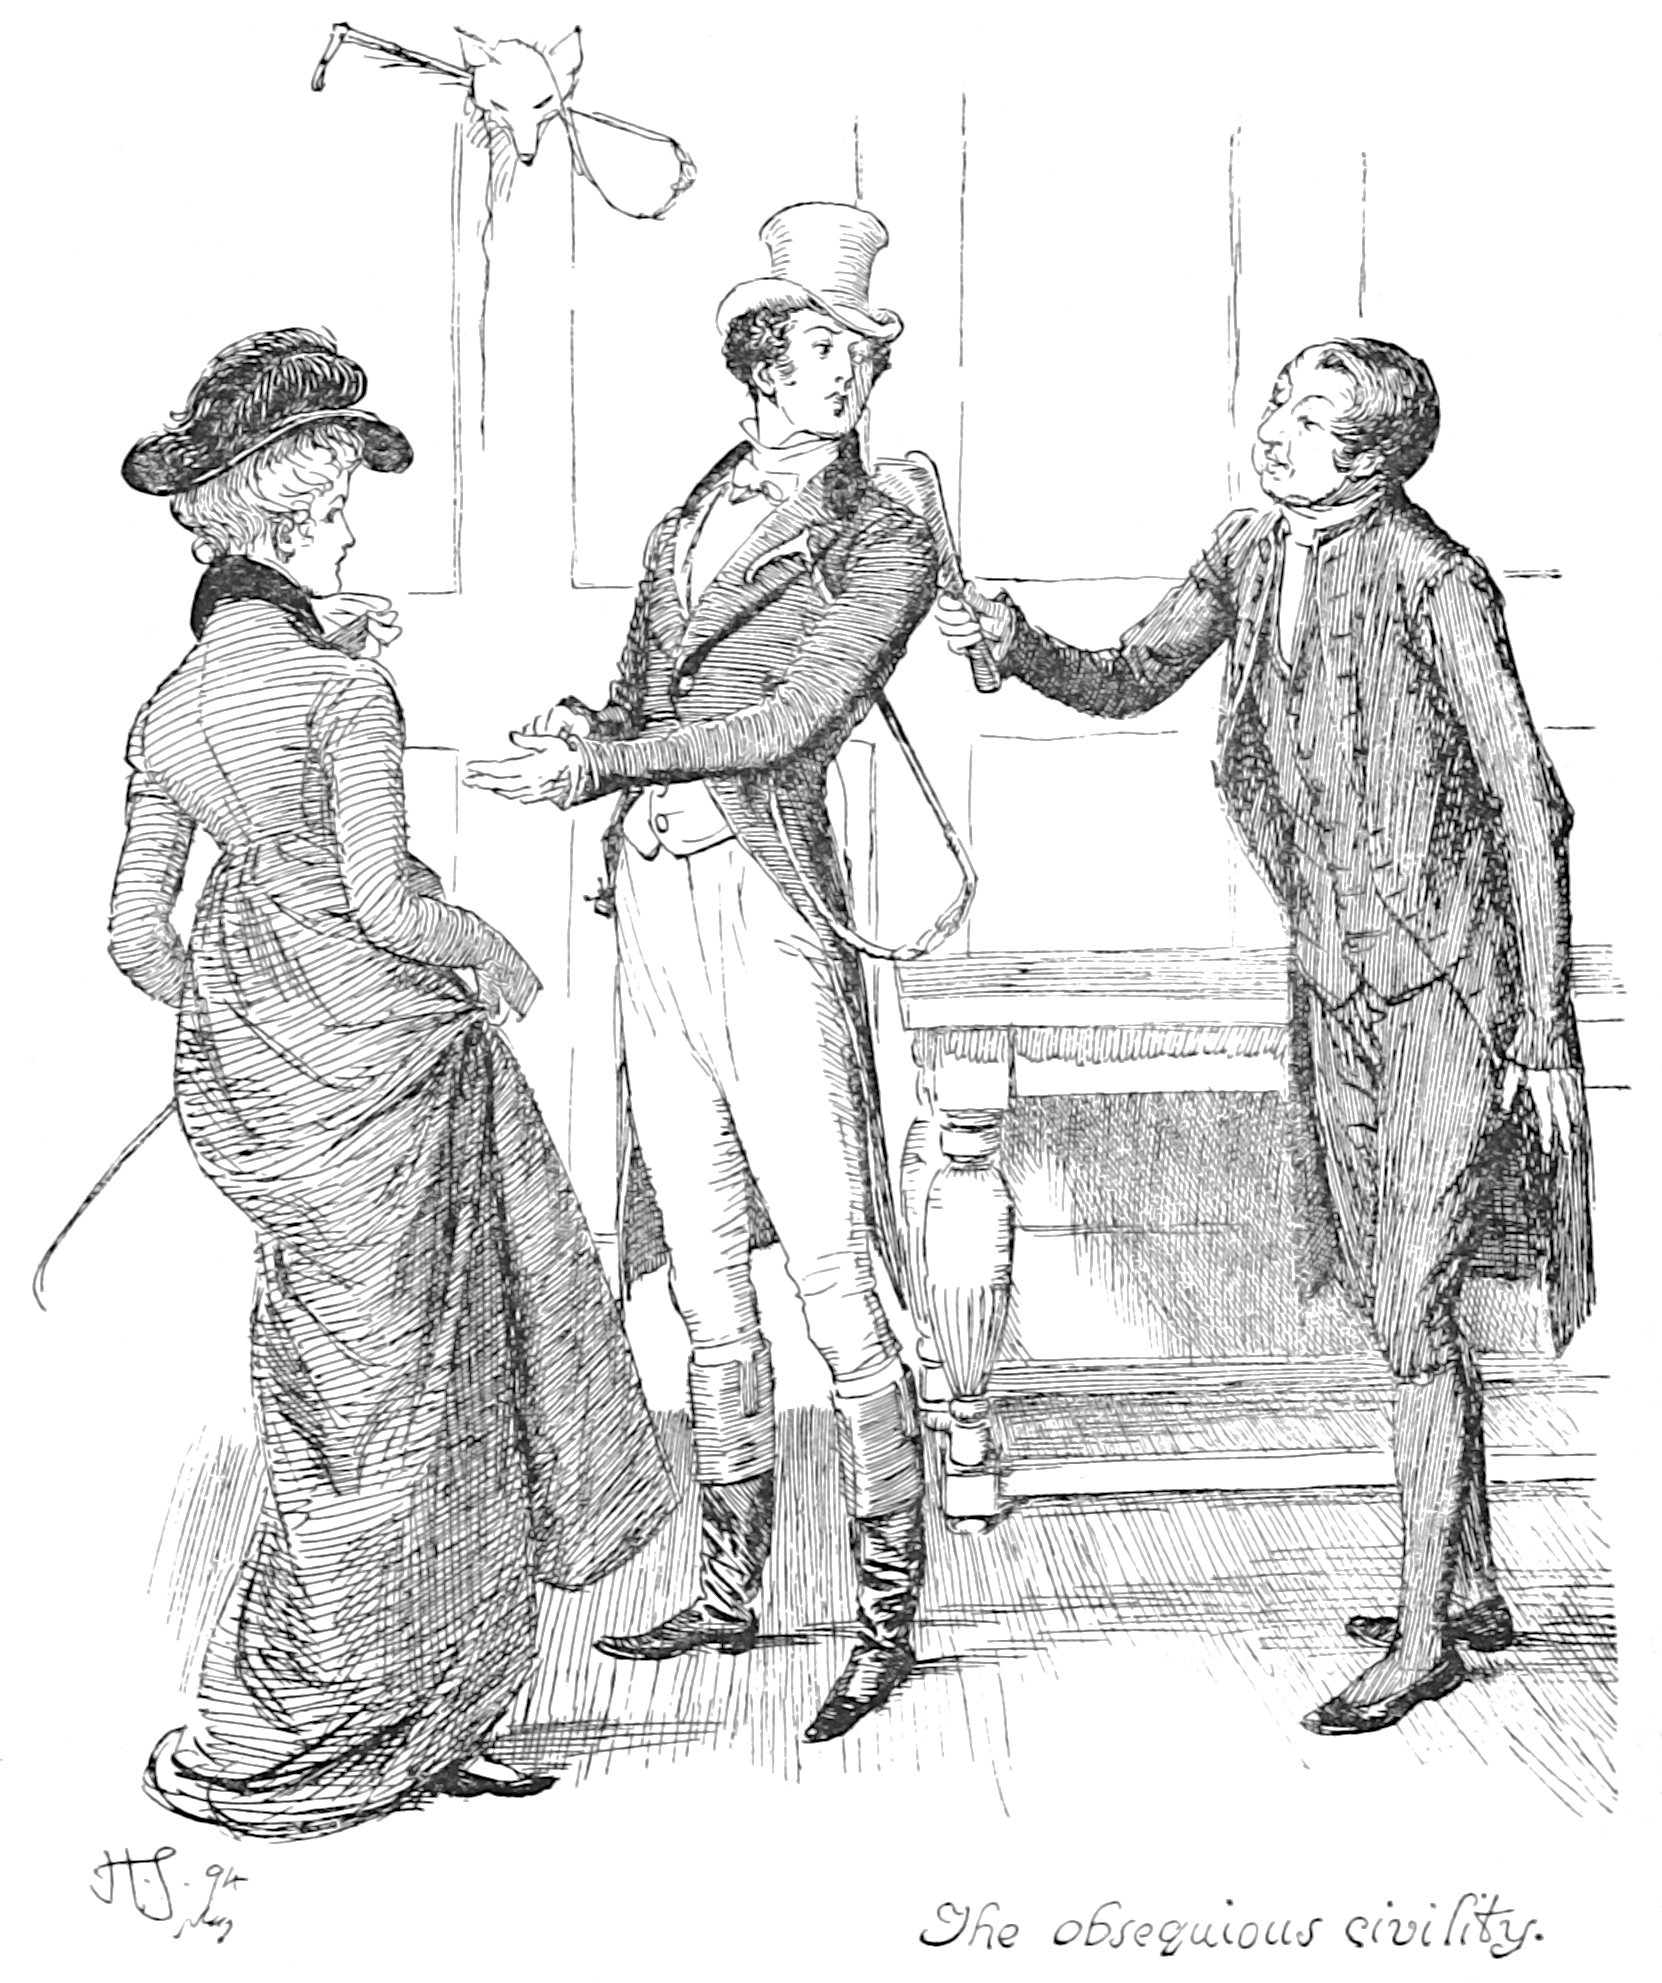
\includegraphics[width=.8\linewidth]{60top}
\captionlistentry{The obsequious civility}
\end{figure}


\lettrine[lines=6,image=true]{initials/chap60e}{lizabeth's} spirits soon rising to playfulness again, she wanted Mr Darcy to account for his having ever fallen in love with her. »How could you begin?« said she. »I can comprehend your going on charmingly, when you had once made a beginning; but what could set you off in the first place?«

\zz
»I cannot fix on the hour, or the spot, or the look, or the words, which laid the foundation. It is too long ago. I was in the middle before I knew that I \textit{had} begun.«

»My beauty you had early withstood, and as for my manners—my behaviour to \textit{you} was at least always bordering on the uncivil, and I never spoke to you without rather wishing to give you pain than not. Now, be sincere; did you admire me for my impertinence?«

»For the liveliness of your mind I did.«

»You may as well call it impertinence at once. It was very little less. The fact is, that you were sick of civility, of deference, of officious attention. You were disgusted with the women who were always speaking, and looking, and thinking for \textit{your} approbation alone. I roused and interested you, because I was so unlike \textit{them}. Had you not been really amiable you would have hated me for it: but in spite of the pains you took to disguise yourself, your feelings were always noble and just; and in your heart you thoroughly despised the persons who so assiduously courted you. There—I have saved you the trouble of accounting for it; and really, all things considered, I begin to think it perfectly reasonable. To be sure you know no actual good of me—but nobody thinks of \textit{that} when they fall in love.«

»Was there no good in your affectionate behaviour to Jane, while she was ill at Netherfield?«

»Dearest Jane! who could have done less for her? But make a virtue of it by all means. My good qualities are under your protection, and you are to exaggerate them as much as possible; and, in return, it belongs to me to find occasions for teasing and quarrelling with you as often as may be; and I shall begin directly, by asking you what made you so unwilling to come to the point at last? What made you so shy of me, when you first called, and afterwards dined here? Why, especially, when you called, did you look as if you did not care about me?«

»Because you were grave and silent, and gave me no encouragement.«

»But I was embarrassed.«

»And so was I.«

»You might have talked to me more when you came to dinner.«

»A man who had felt less might.«

»How unlucky that you should have a reasonable answer to give, and that I should be so reasonable as to admit it! But I wonder how long you \textit{would} have gone on, if you had been left to yourself. I wonder when you \textit{would} have spoken if I had not asked you! My resolution of thanking you for your kindness to Lydia had certainly great effect. \textit{Too much}, I am afraid; for what becomes of the moral, if our comfort springs from a breach of promise, for I ought not to have mentioned the subject? This will never do.«

»You need not distress yourself. The moral will be perfectly fair. Lady Catherine's unjustifiable endeavours to separate us were the means of removing all my doubts. I am not indebted for my present happiness to your eager desire of expressing your gratitude. I was not in a humour to wait for an opening of yours. My aunt's intelligence had given me hope, and I was determined at once to know everything.«

»Lady Catherine has been of infinite use, which ought to make her happy, for she loves to be of use. But tell me, what did you come down to Netherfield for? Was it merely to ride to Longbourn and be embarrassed? or had you intended any more serious consequences?«

»My real purpose was to see \textit{you}, and to judge, if I could, whether I might ever hope to make you love me. My avowed one, or what I avowed to myself, was to see whether your sister was still partial to Bingley, and if she were, to make the confession to him which I have since made.«

»Shall you ever have courage to announce to Lady Catherine what is to befall her?«

»I am more likely to want time than courage, Elizabeth. But it ought to be done; and if you will give me a sheet of paper it shall be done directly.«

»And if I had not a letter to write myself, I might sit by you, and admire the evenness of your writing, as another young lady once did. But I have an aunt, too, who must not be longer neglected.«

From an unwillingness to confess how much her intimacy with Mr Darcy had been overrated, Elizabeth had never yet answered Mrs Gardiner's long letter; but now, having \textit{that} to communicate which she knew would be most welcome, she was almost ashamed to find that her uncle and aunt had already lost three days of happiness, and immediately wrote as follows:—

\begin{quotation}

\indent I would have thanked you before, my dear aunt, as I ought to have done, for your long, kind, satisfactory detail of particulars; but, to say the truth, I was too cross to write. You supposed more than really existed. But \textit{now} suppose as much as you choose; give a loose to your fancy, indulge your imagination in every possible flight which the subject will afford, and unless you believe me actually married, you cannot greatly err. You must write again very soon, and praise him a great deal more than you did in your last. I thank you again and again, for not going to the Lakes. How could I be so silly as to wish it! Your idea of the ponies is delightful. We will go round the park every day. I am the happiest creature in the world. Perhaps other people have said so before, but no one with such justice. I am happier even than Jane; she only smiles, I laugh. Mr Darcy sends you all the love in the world that can be spared from me. You are all to come to Pemberley at Christmas.\\

\begin{flushright}
Yours, etc.
\end{flushright}
\end{quotation}



Mr Darcy's letter to Lady Catherine was in a different style, and still different from either was what Mr Bennet sent to Mr Collins, in return for his last.

\begin{quotation}
\noindent Dear Sir,\\

\indent I must trouble you once more for congratulations. Elizabeth will soon be the wife of Mr Darcy. Console Lady Catherine as well as you can. But, if I were you, I would stand by the nephew. He has more to give.

\begin{flushright}
Yours sincerely, etc.
\end{flushright}
\end{quotation}


Miss Bingley's congratulations to her brother on his approaching marriage were all that was affectionate and insincere. She wrote even to Jane on the occasion, to express her delight, and repeat all her former professions of regard. Jane was not deceived, but she was affected; and though feeling no reliance on her, could not help writing her a much kinder answer than she knew was deserved.

The joy which Miss Darcy expressed on receiving similar information was as sincere as her brother's in sending it. Four sides of paper were insufficient to contain all her delight, and all her earnest desire of being loved by her sister.

Before any answer could arrive from Mr Collins, or any congratulations to Elizabeth from his wife, the Longbourn family heard that the Collinses were come themselves to Lucas Lodge. The reason of this sudden removal was soon evident. Lady Catherine had been rendered so exceedingly angry by the contents of her nephew's letter, that Charlotte, really rejoicing in the match, was anxious to get away till the storm was blown over. At such a moment, the arrival of her friend was a sincere pleasure to Elizabeth, though in the course of their meetings she must sometimes think the pleasure dearly bought, when she saw Mr Darcy exposed to all the parading and obsequious civility of her husband. He bore it, however, with admirable calmness. He could even listen to Sir William Lucas, when he complimented him on carrying away the brightest jewel of the country, and expressed his hopes of their all meeting frequently at St James's, with very decent composure. If he did shrug his shoulders, it was not till Sir William was out of sight.

Mrs Philips's vulgarity was another, and, perhaps, a greater tax on his forbearance; and though Mrs Philips, as well as her sister, stood in too much awe of him to speak with the familiarity which Bingley's good-humour encouraged; yet, whenever she \textit{did} speak, she must be vulgar. Nor was her respect for him, though it made her more quiet, at all likely to make her more elegant. Elizabeth did all she could to shield him from the frequent notice of either, and was ever anxious to keep him to herself, and to those of her family with whom he might converse without mortification; and though the uncomfortable feelings arising from all this took from the season of courtship much of its pleasure, it added to the hope of the future; and she looked forward with delight to the time when they should be removed from society so little pleasing to either, to all the comfort and elegance of their family party at Pemberley.